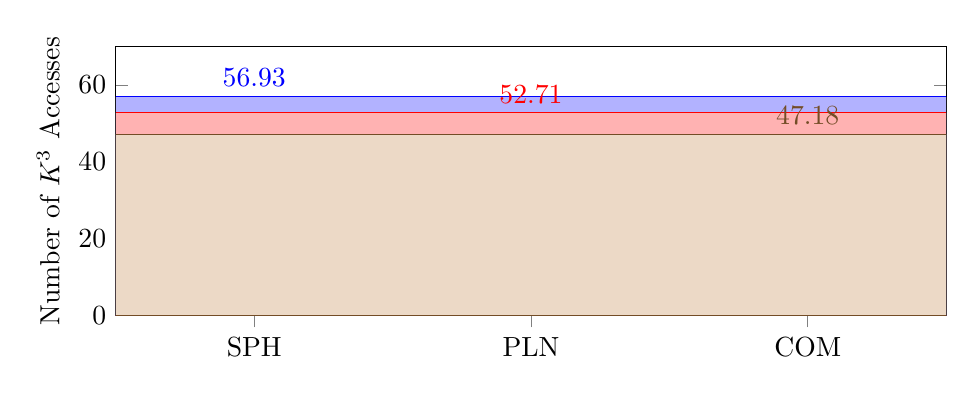
\begin{tikzpicture}
    \begin{axis}[
    ybar,
    width=\linewidth, height=5cm,
    ylabel={Number of $K^3$ Accesses}, ylabel near ticks, ymin=0, ymax=70,
    xticklabels={SPH, PLN, COM},
    xtick={1, 2, 3}, xmin=0.5, xmax=3.5, xtick pos=left,
    nodes near coords, nodes near coords align={vertical},
    every axis plot/.append style={
    ybar,
    bar width=40,
    bar shift=0pt,
    fill
    }
    ]
        \addplot coordinates {(1, 56.93)}; % SPH
        \addplot coordinates {(2, 52.71)}; % PLN
        \addplot coordinates {(3, 47.18)};
    \end{axis}
\end{tikzpicture}

%SELECT AVG(QueryCount), IdentificationMethod
%FROM REDUCTION
%WHERE rowid IN (
%    SELECT rowid
%    FROM REDUCTION
%    WHERE (IdentificationMethod LIKE 'Plane' OR IdentificationMethod LIKE 'Sphere')
%    AND ShiftDeviation < 1.0e-3 AND ShiftDeviation > 1.0e-5 AND FalseStars = 0
%    AND QueryCount > 1
%)
%GROUP BY IdentificationMethod

%SELECT AVG(QueryCount)
%FROM REDUCTION
%WHERE rowid IN (
%    SELECT rowid
%    FROM REDUCTION
%    WHERE IdentificationMethod LIKE 'Composite'
%    AND ShiftDeviation < 1.0e-3 AND ShiftDeviation > 1.0e-5 AND FalseStars = 0
%    AND QueryCount > 1
%)